%%%%%%%%%%%%%%%%%%%%%%%%%%%%%%%%%%%%%%%%%
% a0poster Landscape Poster
% LaTeX Template
% Version 1.0 (22/06/13)
%
% The a0poster class was created by:
% Gerlinde Kettl and Matthias Weiser (tex@kettl.de)
% 
% This template has been downloaded from:
% http://www.LaTeXTemplates.com
%
% License:
% CC BY-NC-SA 3.0 (http://creativecommons.org/licenses/by-nc-sa/3.0/)
%
%%%%%%%%%%%%%%%%%%%%%%%%%%%%%%%%%%%%%%%%%

%----------------------------------------------------------------------------------------
%	PACKAGES AND OTHER DOCUMENT CONFIGURATIONS
%----------------------------------------------------------------------------------------

\documentclass[a0,landscape]{a0poster}

\usepackage{multicol} % This is so we can have multiple columns of text side-by-side
\columnsep=100pt % This is the amount of white space between the columns in the poster
\columnseprule=7pt % This is the thickness of the black line between the columns in the poster

\usepackage[svgnames]{xcolor} % Specify colors by their 'svgnames', for a full list of all colors available see here: http://www.latextemplates.com/svgnames-colors

\usepackage{times} % Use the times font
%\usepackage{palatino} % Uncomment to use the Palatino font

\usepackage{graphicx} % Required for including images
\graphicspath{{figures/}} % Location of the graphics files
\usepackage{booktabs} % Top and bottom rules for table
\usepackage[font=large,labelfont=bf]{caption} % Required for specifying captions to tables and figures
\usepackage{amsfonts, amsmath, amsthm, amssymb} % For math fonts, symbols and environments
\usepackage{wrapfig} % Allows wrapping text around tables and figures
\usepackage{comment}
\usepackage{bm}
\usepackage{anyfontsize}
\usepackage{multirow}

\usepackage{sidecap}

\newcommand{\mysection}[1]{\section*{\fontsize{67.1}{82} \selectfont \color{NavyBlue} #1 \color{Black}}}

\renewcommand{\vec}[1]{{\boldsymbol{\mathbf{#1}}}} % vector
\newcommand{\mat}[1]{{\ensuremath{\mathbf{#1}}}} % matrix

\newcommand{\R}{\mathbb{R}}
\newcommand{\D}{\mathcal{D}}
\newcommand{\N}{\mathcal{N}}
\newcommand{\set}[1]{\mathcal{#1}}

\newcommand{\bigO}{\mathcal{O}}
\newcommand{\ceq}{{\stackrel{c}{=}}}
\newcommand{\half}{\frac{1}{2}}
\newcommand{\T}{^\top}
\newcommand{\I}{\mathbb{I}}

\newcommand{\grad}{\nabla}
\newcommand{\sample}{\sim}
\newcommand{\given}{|}

\newcommand{\norm}{\mathcal{N}}
\newcommand{\bern}{\textrm{Bern}}

\DeclareMathOperator*{\argmin}{argmin}
\DeclareMathOperator*{\argmax}{argmax}

\newcommand{\target}{{p^\star}}
\newcommand{\prop}{q}
\newcommand{\pinit}{{p_0}}

\newcommand{\PG}{{p_G}}
\newcommand{\PD}{{p_D}}
\newcommand{\PR}{{p_{\textrm{data}}}}
\newcommand{\accept}{\alpha}

\newcommand{\setx}{\set{X}}

\newcommand{\bmu}{\boldsymbol{\mu}}
\newcommand{\bK}{\boldsymbol{\mathrm{K}}}
\newcommand{\bM}{\boldsymbol{\mathrm{M}}}
\newcommand{\mbf}[1]{{\boldsymbol{\mathbf{#1}}}}
\renewcommand{\bm}{\mbf}

\usepackage{subfigure}

\usepackage{parskip}

\usepackage{url}

\usepackage{float} 

\usepackage{array}
\newcolumntype{P}[1]{>{\centering\arraybackslash}p{#1}}

\begin{document}

%----------------------------------------------------------------------------------------
%	POSTER HEADER 
%----------------------------------------------------------------------------------------

% The header is divided into three boxes:
% The first is 55% wide and houses the title, subtitle, names and university/organization
% The second is 25% wide and houses contact information
% The third is 19% wide and houses a logo for your university/organization or a photo of you
% The widths of these boxes can be easily edited to accommodate your content as you see fit

{
\setlength\extrarowheight{35pt}
\begin{tabular}{P{15cm}cP{15cm}}
~ &
{\fontsize{100}{120} \selectfont \color{NavyBlue} \textbf{Metropolis-Hastings Generative Adversarial Networks} \color{Black}}
&

\includegraphics[width=10cm]{uber_ai_logo_bootleg.pdf} \\
~ &
\Huge \textbf{Ryan Turner, Jane Hung, Yunus Saatci, Jason Yosinski} &
~
\end{tabular}
}
%
\vspace{2cm} % A bit of extra whitespace between the header and poster content

%----------------------------------------------------------------------------------------

\begin{multicols}{3} % This is how many columns your poster will be broken into, a poster with many figures may benefit from less columns whereas a text-heavy poster benefits from more

%----------------------------------------------------------------------------------------
%	INTRODUCTION
%----------------------------------------------------------------------------------------

\Large

\mysection{Why Resample GANs?}

\begin{itemize}
  \item GANs can estimate densities differently than traditional methods: implicitly without a tractable likelihood
  \item GANs consist of two neural networks, generator $G$ and discriminator $D$, competing against each other
  \item $D$ usually thrown away $\implies$ use new method to capture knowledge in $D$: wrap $G$ and create a more intelligent $G'$
\end{itemize}
%
\begin{align}
  D(\vec x) = \frac{\PD(\vec x)}{\PD(\vec x) + \PG(\vec x)}
\end{align}
%
\begin{itemize}
  \item Use MCMC \emph{independence sampler} to sample from implied $\PD$ by taking multiple samples from $G$
  \item Amazingly: given a perfect $D$ and imperfect $G$, still obtain exact samples from true data distribution $\PR$
  \item Can avoid the need for densities needed in typical MCMC
\end{itemize}
%
\begin{align}
  \frac{\PD(\vec x)}{\PG(\vec x)} = \frac{D(\vec x)}{1 - D(\vec x)}
\end{align}
%
~\\
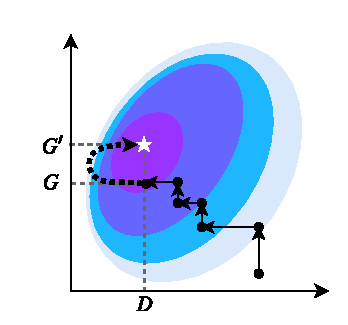
\includegraphics[scale=2.75]{../figures/coord_descent.pdf}
\hspace{7mm}
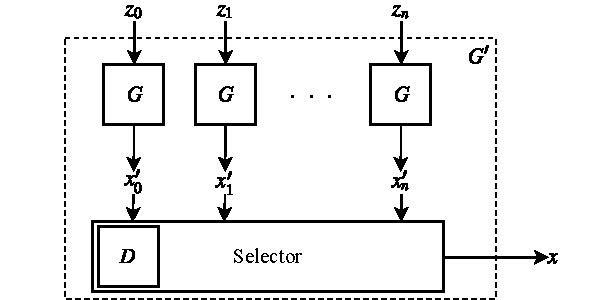
\includegraphics[scale=2.75]{../figures/block_diag.pdf}
\vspace{-2cm}

\mysection{Rejection Sampling}

\begin{itemize}
  \item Discriminator Rejection Sampling (DRS) also corrects $G$ using the probabilities given by $D$
  \item Rejection sampling uses $\accept = p_D/(Mp_G)$ with $M$ s.t.~$\alpha \leq 1$
  \item $M$ must be estimated from many pilot samples
  \item Very low acceptance probabilities in high dimensions without $\gamma$-shift heuristic
  \item $\gamma$-shift heuristic violates rejection sampling validity
  \item We use MCMC instead: invented as replacement for rejection sampling in high dimensions
\end{itemize}

\columnbreak

\mysection{Metropolis-Hastings}

\begin{itemize}
  \item Samples $\vec x_{1:K} \in \setx^K$ marginally from target $\target$
  \item Use independence sampler as $\vec x' \sample \prop(\vec x' \given \vec x_k)=\prop(\vec x')$
  \item Accept with probability:
  \begin{align}
    \accept(\vec x', \vec x_k) = \min\left(1, \frac{\target(\vec x')\prop(\vec x_k)}{\target(\vec x_k)\prop(\vec x')}\right) \in [0,1]\,. \label{eq:alpha def}
  \end{align}
  \item Independent samples: $\vec x_0 \sample \pinit$ and then $K$ MH steps for $\vec x_K$ as output
  \item Detailed balance: $\vec x_k \sample \target \implies \vec x_{k+1} \sample \target$, initialize as close to $\target$ as possible
\end{itemize}

\mysection{MH-GAN Practical Details}

\begin{itemize}
  \item Implicit model on $\vec x$ via \smash{$G \in \R^{d} \rightarrow \setx$}:
  \begin{align}
    \vec x = G(\vec z)\,, \quad \vec z \sample \norm(\vec 0, \vec I_{d})\,.
  \end{align}
  \item Generator distribution $\vec x \sample \PG$, implied discriminator distribution $\PD$, unknown true distribution $\PR$
  \item If $D$ and $G$ converge: $\PD = \PR = \PG$
  \item If $D$ optimal for fixed $G$: $\PD = \PR \neq \PG$
\end{itemize}

Sample from $\PD$:
\begin{align}
  \frac{\PD}{\PG} = \frac{1}{D^{-1} - 1} \implies
  \accept(\vec x', \vec x_k) = \min\left(1, \frac{D(\vec x_k)^{-1} - 1}{D(\vec x')^{-1} - 1}\right)
\end{align}
If $D$ is perfect $\PD = \PR$ (perfect target distribution)

Modifications:
\begin{itemize}
  \item $D$ must be well calibrated to build valid $\accept$ $\implies$ Correct using isotonic regression on held out data
  \item Avoid burn-in by initialization: sample from \emph{data} distribution $\PR$ $\implies$ initialize at real sample
\end{itemize}

Weaken perfect $D$ assumption:
\begin{itemize}
  \item Apply recalibration $\implies$ probabilities need not be correct
  \item $D$ only needs to be correct on $\PG$ and $\PR$ manifold.
\end{itemize}

\columnbreak

\mysection{Results}

Consider 1D example to illustrate procedure
\begin{center}
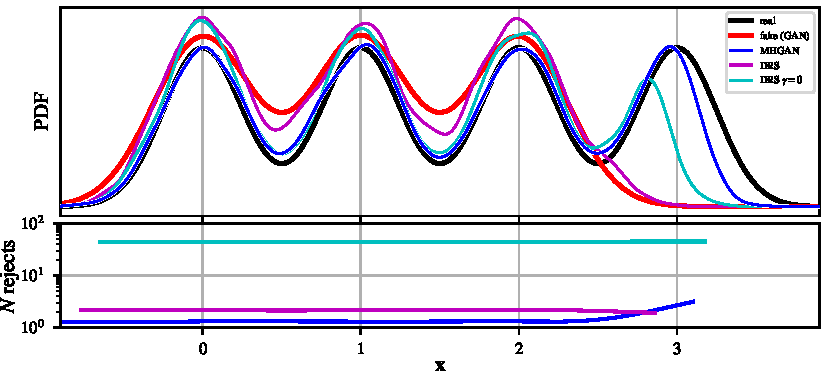
\includegraphics[scale=2.5]{../figures/univariate_example.pdf}
\end{center}
Use 25 Gaussians example using trained GAN:
\begin{center}
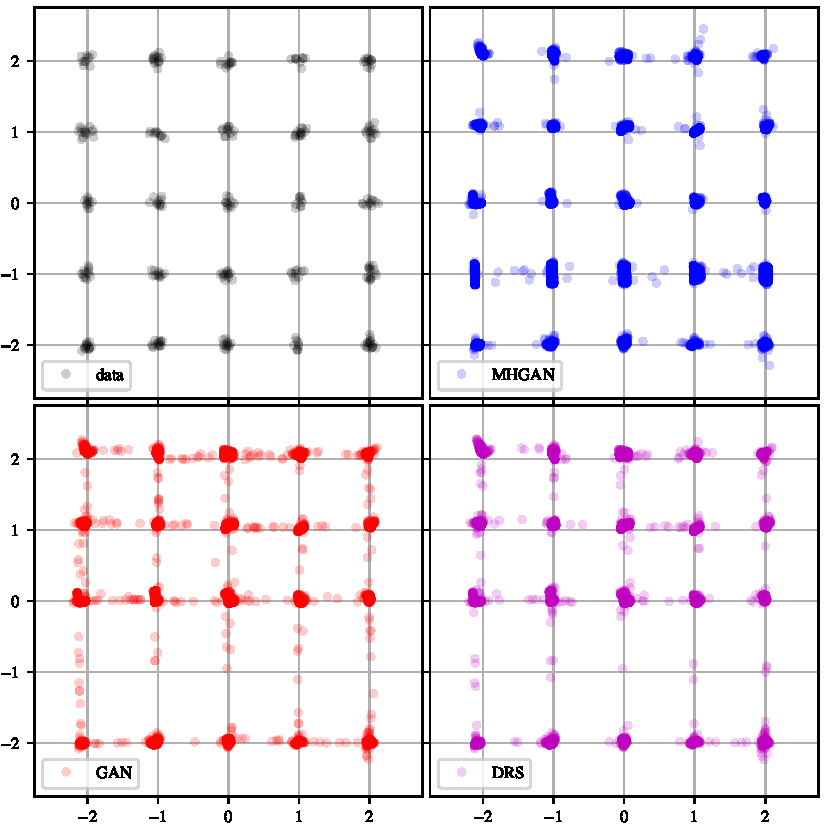
\includegraphics[scale=1.0]{../figures/mog_example_150.pdf}
\hspace{7mm}
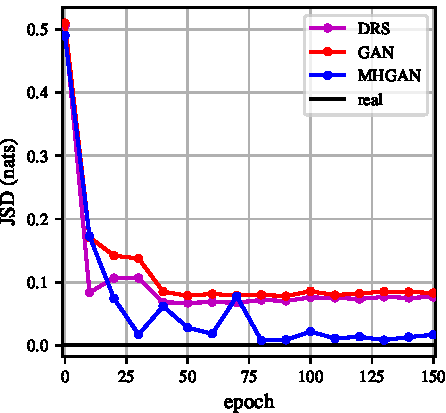
\includegraphics[scale=2.0]{../figures/jsd.pdf}
\end{center}
Comparison on real data using CIFAR-10:
\begin{center}
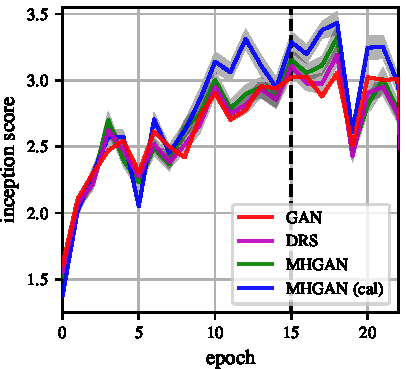
\includegraphics[scale=2.5]{../figures/per_epoch.pdf}
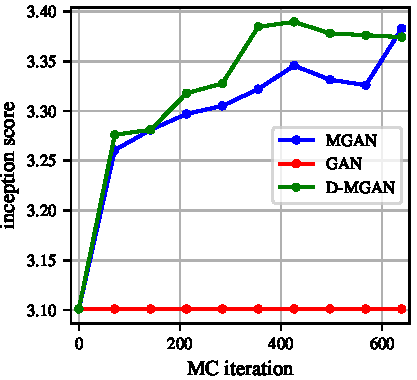
\includegraphics[scale=2.5]{../figures/plot_per_mh.pdf}
\end{center}

\paragraph{Code}
\centering
\large {\url{github.com/uber-research/metropolis-hastings-gans}}

\end{multicols}
\end{document}

